\documentclass[10pt]{article}

\usepackage{graphicx}			% Use this package to include images
\usepackage{amsmath}			% A library of many standard math expressions
\usepackage{amsfonts}
\usepackage[margin=1in]{geometry}% Sets 1in margins.
\usepackage{fancyhdr}			% Creates headers and footers
\usepackage{enumerate}          %These two package give custom labels to a list
\usepackage[shortlabels]{enumitem}
\usepackage{braket}
\usepackage{physics}
\usepackage{pgfplots}
\usepackage{tikz}
\usepackage{xcolor}
\usepackage{mathtools}
\usepackage{url}
\usepackage{listings}
\usepackage{geometry}
\usepackage{titling}

%% LISTINGS CONFIG %%

\definecolor{purple2}{RGB}{153,0,153} % there's actually no standard purple
\definecolor{green2}{RGB}{0,153,0} % a darker green

\lstset{
  language=Python,                   % the language
  basicstyle=\ttfamily\small,   % size of the fonts for the code
  frame = single,
  % Color settings to match IDLE style
  keywordstyle=\color{orange},       % core keywords
  keywordstyle={[2]\color{purple2}}, % built-ins
  stringstyle=\color{green2},%
  showstringspaces=false,
  commentstyle=\color{red},%
  upquote=true,                      % requires textcomp
  numbers=left,
  breaklines=true,
}

\setlength{\droptitle}{-6em}     % Eliminate the default vertical space

\title{\textbf{ECE469 - Introduction to ML} \\ \textit{Midterm - Part 1}}
\author{Chase A. Lotito - \textit{SIUC Undergraduate}}
\date{\today}

\begin{document} %The writing for your homework should all come after this.

\maketitle


% QUESTION 1
\textbf{Question 1.} \textit{Regression in machine learning.}

\bigskip
\textbf{Solution.}

% 1.a
\smallskip
\textit{(A)}
\begin{figure}[h]
    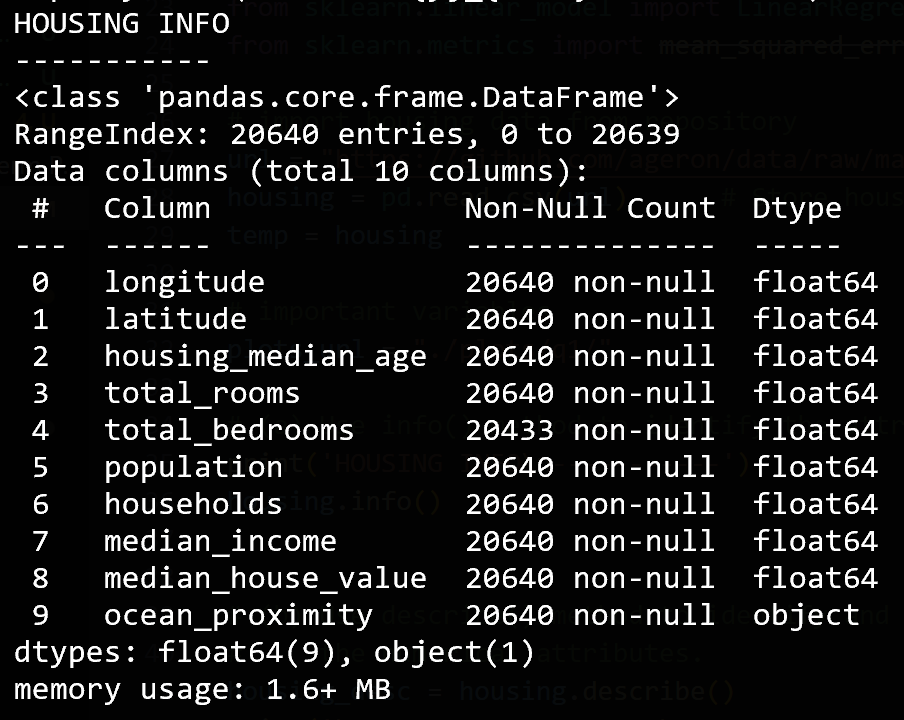
\includegraphics[width=0.6\textwidth]{../logs/housing_info.png}
    \centering
    \caption{housing.info()}
\end{figure}

% 1.b
\smallskip
\textit{(B)}
\begin{figure}[h]
    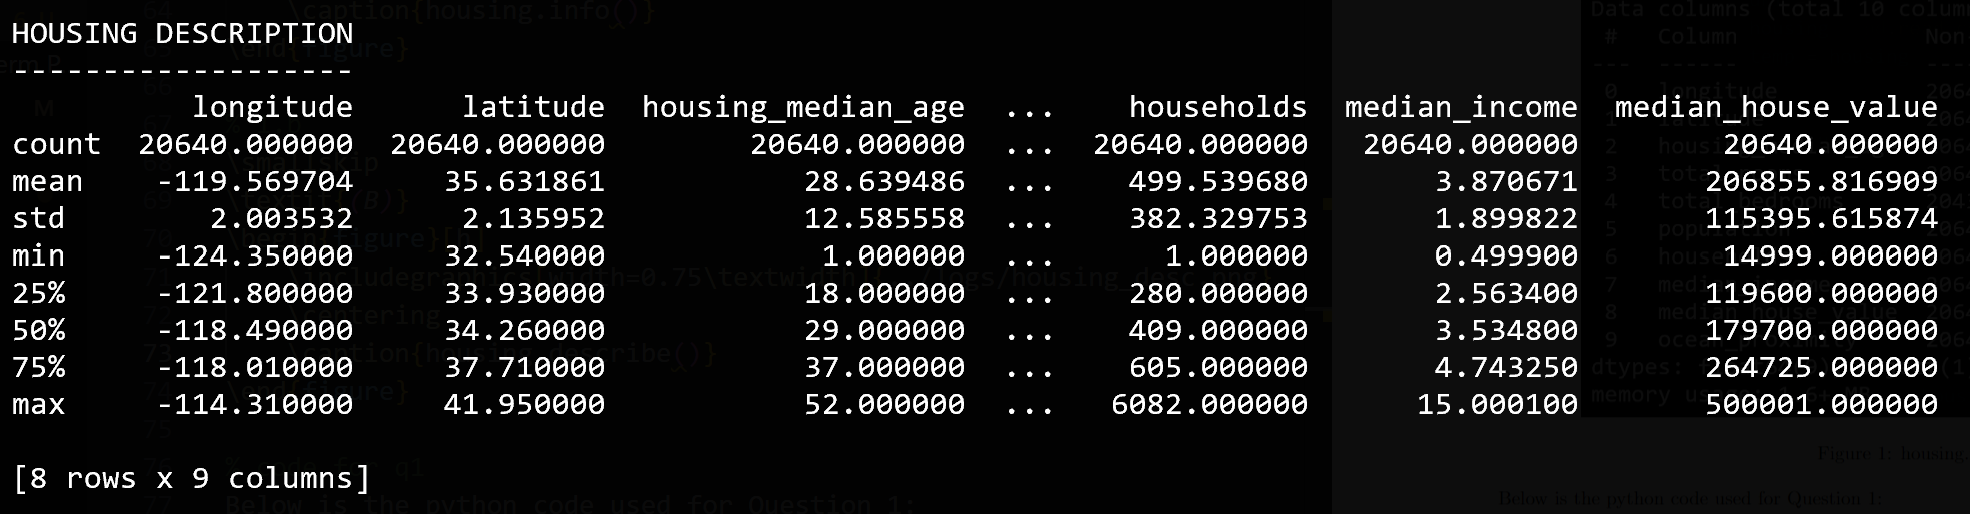
\includegraphics[width=0.85\textwidth]{../logs/housing_desc.png}
    \centering
    \caption{housing.describe()}
\end{figure}

\clearpage

% 1.c
\smallskip
\textit{(C)}
\begin{figure}[h]
    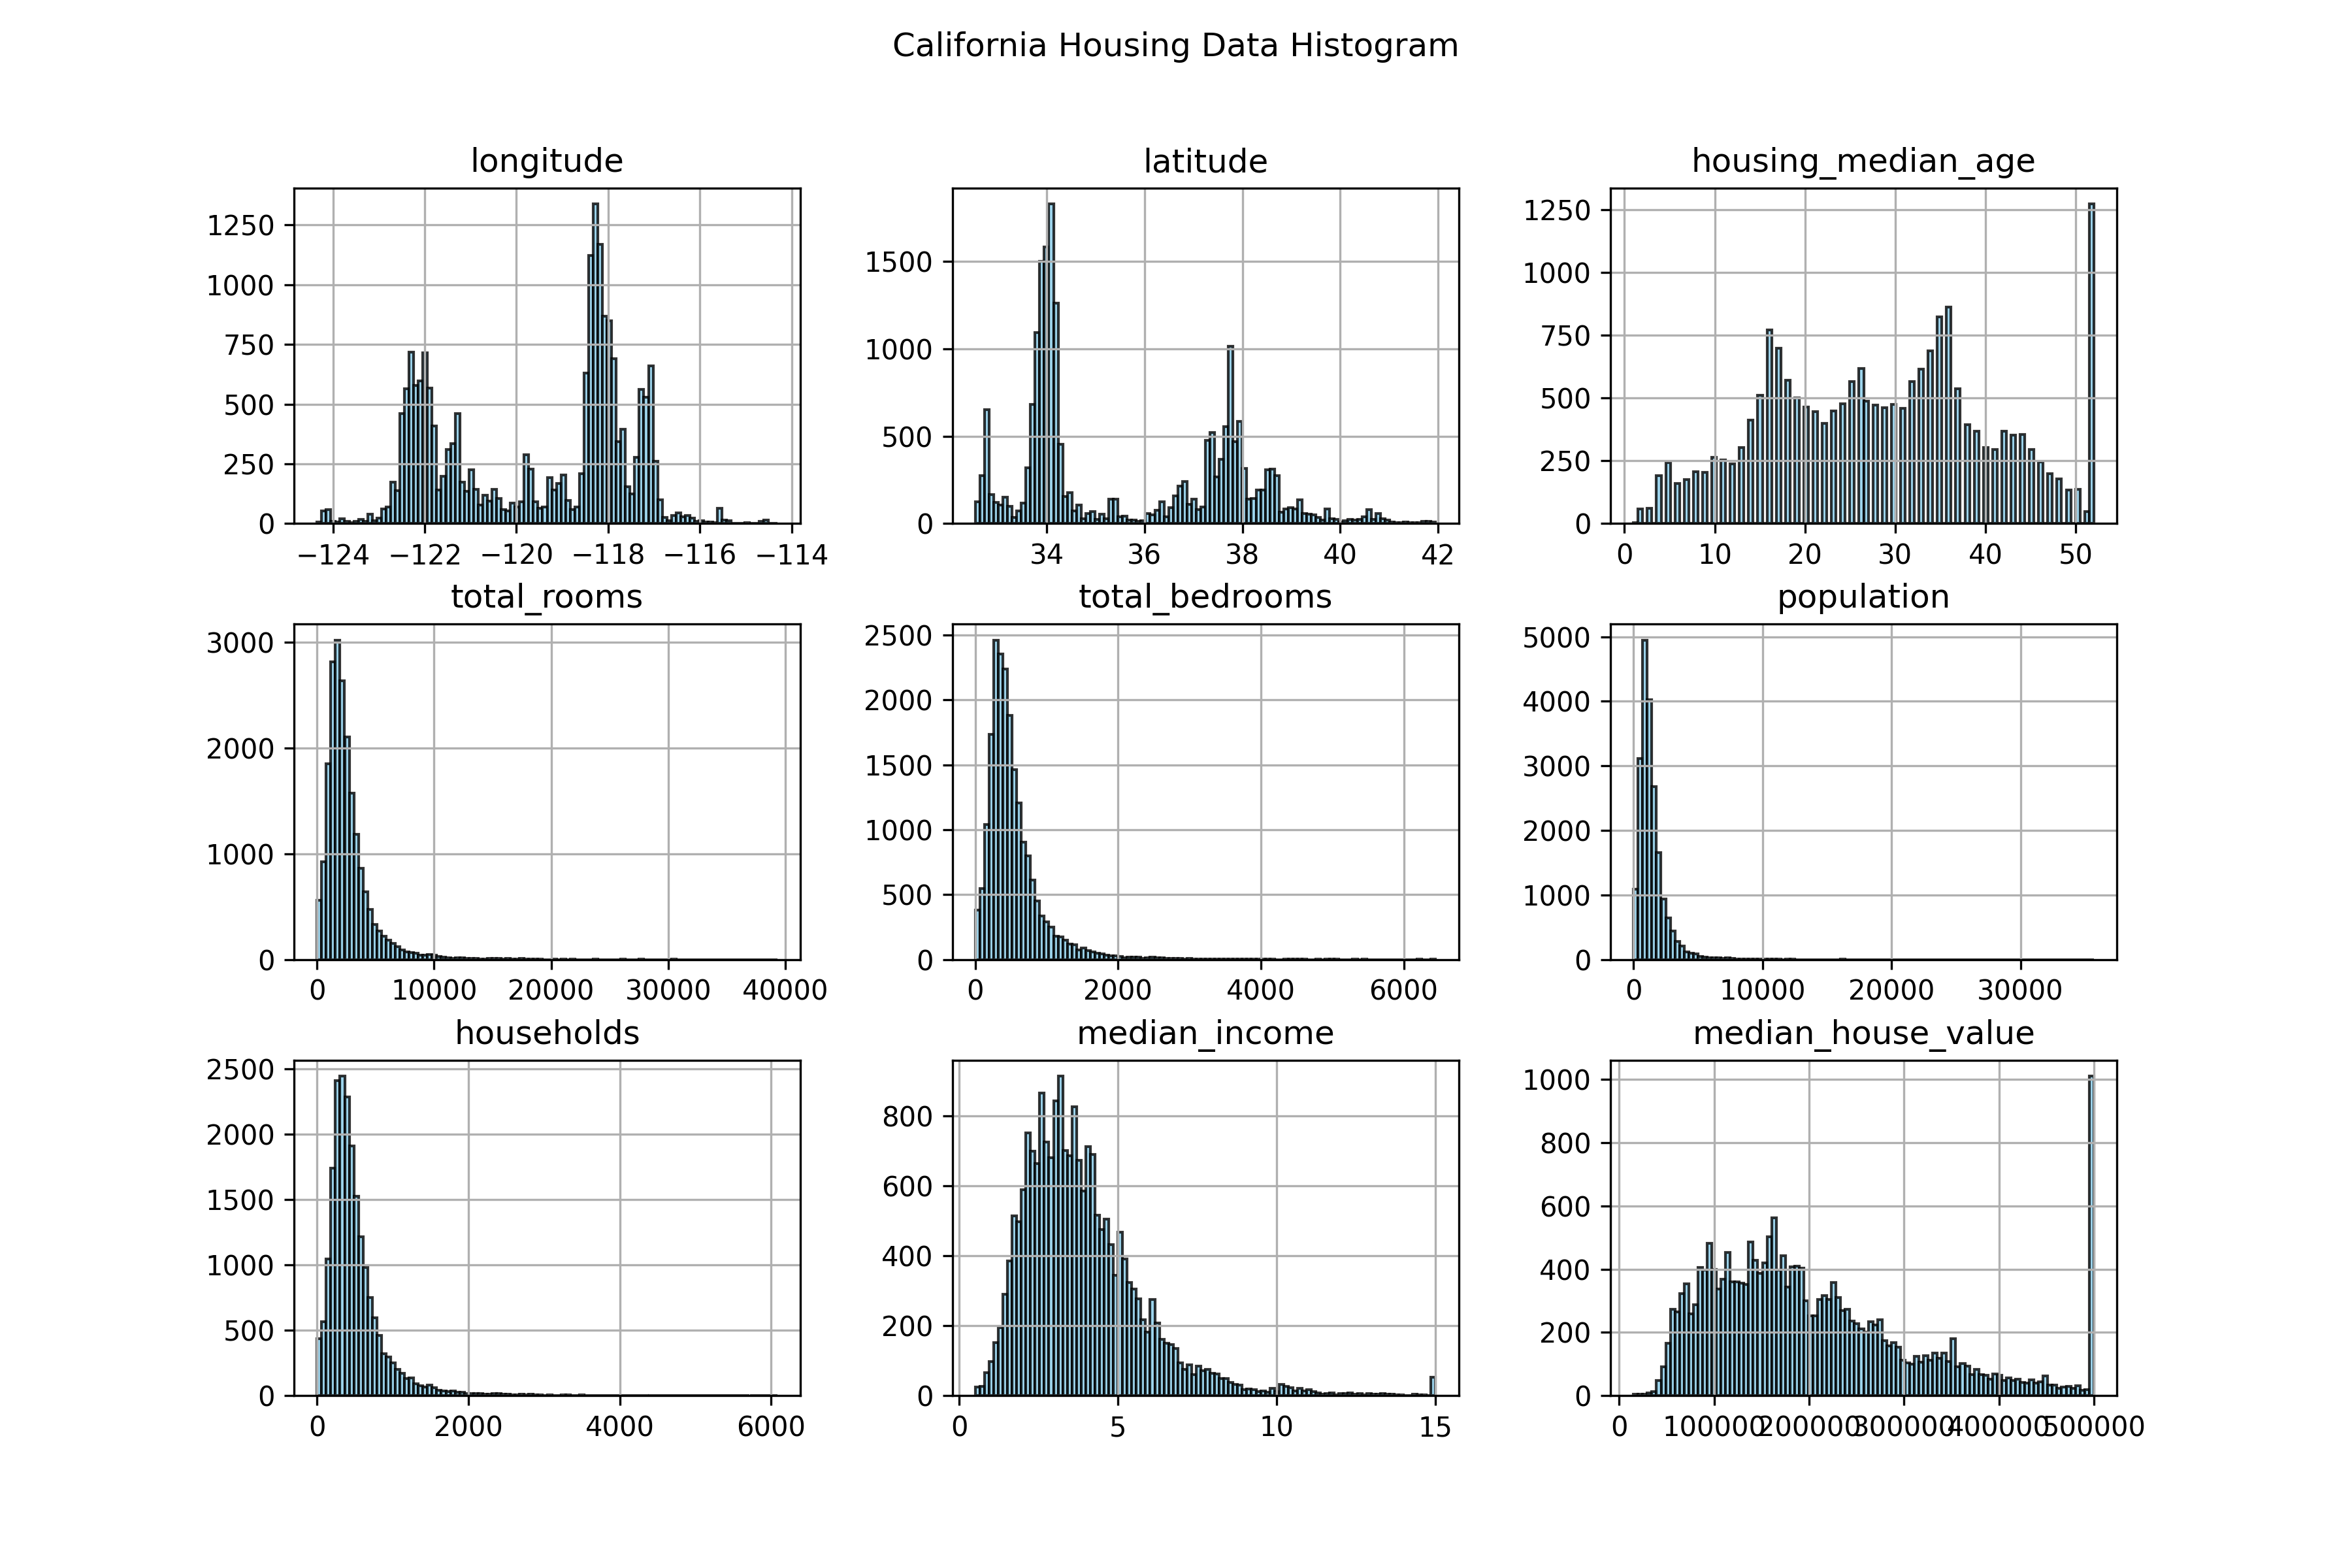
\includegraphics[width=0.95\textwidth]{../plots/q1/housing_histogram.png}
    \centering
    \caption{Housing Dataset Histogram}
\end{figure}

% 1.d
\smallskip
\textit{(D)}

Using \textit{SimpleImputer} from SciKit-Learn to replace missing data with the median value, and using \textit{StandardScaler} from SciKit-Learn to standardize the dataset, the dataset looks as follows:

\begin{figure}[h]
    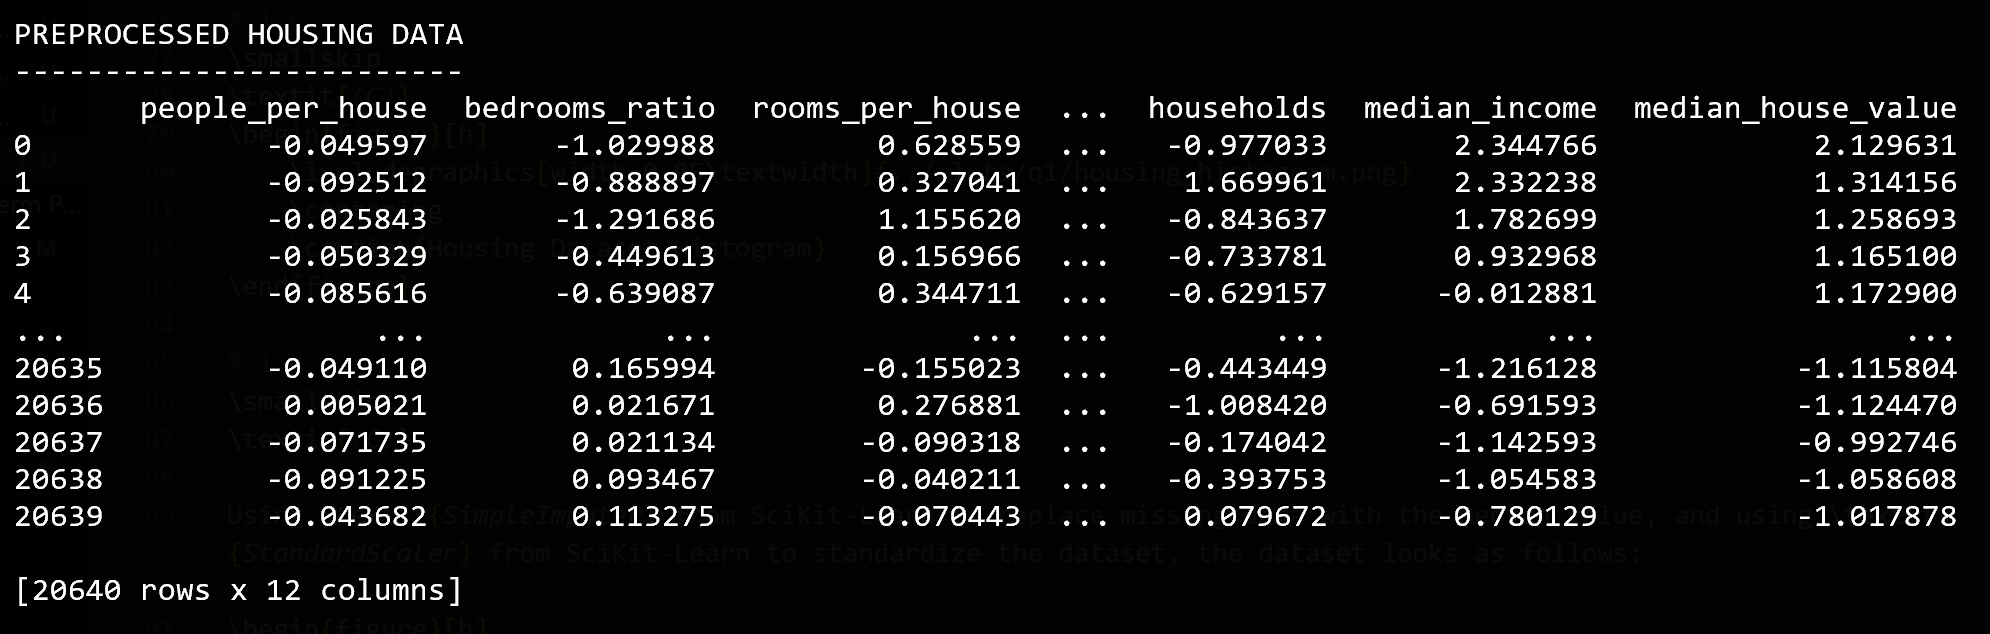
\includegraphics[width=0.85\textwidth]{../logs/housing_pre.png}
    \centering
    \caption{Preprocessed dataset}
\end{figure}

% code for q1
Below is the python code used for Question 1:
\lstinputlisting[caption={File: q1.py}]{../q1.py}

% QUESTION 2
\textbf{Question 2.} \textit{Classification in machine learning.}

\textbf{Solution.}

% code for q2
Below is the python code used for Question 2:
\lstinputlisting[caption={File: q2.py}]{../q2.py}

\end{document}